\documentclass[12pt,reqno,letter]{article}
\usepackage[spanish]{babel}
\usepackage[utf8x]{inputenc}
\usepackage[T1]{fontenc}
\usepackage[table]{xcolor}

\usepackage{graphicx} %allows you to use jpg or png images. PDF is still recommended
\usepackage[colorlinks=False]{hyperref} % add links inside PDF files
\usepackage{amsmath}  % Math fonts
\usepackage{amsfonts} %
\usepackage{amssymb}  %
\usepackage{multicol}
%% Sets page size and margins. You can edit this to your liking
\usepackage[top=1.3cm, bottom=2.0cm, outer=2.5cm, inner=2.5cm, heightrounded,
marginparwidth=1.5cm, marginparsep=0.4cm, margin=2.5cm]{geometry}
%% \usepackage[authoryear]{natbib}
\usepackage[affil-it]{authblk}
%% \bibliographystyle{abbrvnat}
% soporte para UTF-8
\usepackage[utf8x]{inputenc} 
\PrerenderUnicode{ü}
\usepackage{enumitem}

\newenvironment{fig2}[1][\unskip]{}{} %compatibilidad con fig2

\begin{document}
	\title{ Presentaci\'on de Proyecto de Finanzas Cuantitativas}
	\author{Francisco José Álvarez Rojo, Jorge III Altamirano Astorga, Paulina G\'omez Mont Wiechers}
	\affil{Instituto Tecnol\'ogico Autónomo de México}
	\date{Marzo 2019}
	\maketitle
	
	\begin{abstract}
		En este documento contrastaremos la predicción del retorno del IPC utilizando un modelo ARIMA vs. un modelo de Aprendizaje de Máquina donde consideraremos la información de los ``sentimientos'' capturados en los tweets de fuentes periodísticas sobre ciertas palabras clave con el fin de ver cuál es el mejor modelo.
	\end{abstract}

	    
	\begin{multicols}{2}
    \section{Pregunta}
    
    ¿Podemos usar Procesamiento de Lenguaje Natural (\textit{NLP} ) para la mejorar la estimación del retorno del IPC vs. un modelo ARIMA?
	    
        \section{Introducción}
		Utilizando dos enfoques distintos, el primero es un modelo ARIMA utilizando datos históricos de 
		los retornos del IPC, el segundo es un modelo de  Aprendizaje de Máquina con datos del
		``sentimiento'' extraidos de Tweets,
		contrastaremos si los métodos de Aprendizaje de máquina tienen un mejor performance
		vs. los modelos ARIMA para la predicción del rendimiento dirario del IPC.
		Buscaremos encontrar el ``sentimiento'' con la lectura de tweets de medios electr\'onicos e impresos como \textit{El Financiero}, \textit{El Economista} y \textit{El Universal} .
		
		\section{Datos}

        \subsection{Tweets}

        Este proceso sigue dos grandes etapas de experimentación. En primer lugar, se intenta extraer contenido de twitter directamente desde su API, la cual funciona adecuadamente, sin embargo cuenta con un límite de tweets diarios y no proporciona de manera explícita una metodología para obtener tweets con antigüedad mayor a una semana. 
        
        En segundo lugar, se utilizó la librería GetOldTweets3, el cual está basado en el proyecto de Jefferson-Henrique GetOldTweets-python y permite hacer búsquedas detalladas sobre contenido en twitter. Este paquete hace un proceso de Web scrapping que le permite obtener información de twitter simulando a una persona que navega en la interfaz de la red social. 
        
        El paquete permitió que se realizaran búsquedas específicas que proporcionaran a nuestra investigación información relevante. Los parámetros de búsqueda que se utilizaron fueron: QuerySearch (palabra clave a encontrar dentro de tweets), Username (fuente del tweet), setSince (fecha de inicio de búsqueda), setUntil (fecha límite de búsqueda), setMaxTweets (número máximo de tweets a buscar). 
        
        Se crea una lista de palabras clave que representaran temas, organismos o empresas que pudieran impactar directamente sobre el precio del IPC de México. Así mismo se elaboró una lista de fuentes confiables sobre las cuales buscar tweets y evitar información sesgada. 
        
        \textbf{Lista de palabras clave:}
        \begin{enumerate}
        \item America Movil
        \item Banco de México
        \item México
        \item BMV
        \item Bolsa Mexicana de Valores
        \item Bolsa Mexicana
        \item Ipc
        \item Gobierno de México
        \item Walmex
        \item Femsa
        \item Televisa
        \item Grupo México
        \item Banorte
        \item Cemex
        \item Grupo Alfa
        \item Peñoles
        \item Inbursa
        \item Elektra
        \item Mexichem
        \item Bimbo
        \item Arca Continental
        \item Kimberly-Clark
        \item Genomma Lab
        \item Puerto de Liverpool
        \item Grupo Aeroportuario
        \item Banco Compartamos
        \item Alpek
        \item Ica
        \item Tv Azteca
        \item OHL
        \item Maseca
        \item Alsea
        \item Carso
        \item Lala
        \item Banregio
        \item Comercial Mexicana
        \item IEnova
        \item Pinfra
        \item Santander México
        \item Presidente de México
        \item Cetes
        \end{enumerate}

        \textbf{Lista de fuentes:}
        \begin{enumerate}
        \item El Economista
        \item El Financiero
        \item El Universal
        \end{enumerate}
        
        
        Las búsquedas se basadan en todas las combinaciones posibles que se pueden hacer con estas 3 fuentes y estos 41 temas, dando un total de 123 búsquedas. Además, para evitar que un sólo tweet describa el sentimiento respecto a un cierto tema, se extraen 3 tweets por cada combinación tema-fuente, de esta manera se llega a un número total de 369 tweets diarios.


\subsection{Precio IPC}
	    Obtenemos el precio histórico del 4 de Enero de 2016 al 25 de Marzo de 2019 del índice diario de la página \textit{Yahoo! Finance} tomando el precio de ``Cierre Ajustado'' el cual es el Precio de cierre ajustado para dividendos y división de acciones, para el precio de cierre del IPC MEXICO (MXX). 
	    

        \subsection{EDA}
        
        Como cualquier análisis de datos es importante iniciar conociéndolos:
        \begin{center}
        \begin{tabular}{ |c|c|c|c| } 
         \hline
         count  & 1308.0 & 1.308e+03 & 1306.0 \\
         \hline
         mean &  45570.715 & 1.879e+08    & -0.004 \\
             \hline
            std &    2959.270  & 8.189e+07     & 0.853 \\
             \hline
            min  &  37950.968 &  0.00e+00 &    -6.171 \\
             \hline
            25\%  &  43402.067 &  1.442e+08 &   -0.461 \\
             \hline
            50\%    & 45300.8359  & 1.760e+08    & 0.021 \\
             \hline
            75\%    & 48050.900 &  2.149e+08 &     0.509 \\
             \hline
            max &   51713.378 & 6.966e+08   &  3.463 \\
             \hline
         \hline
        \end{tabular}
        \end{center}
        
        Exploramos los datos para observar como es el comportamiento del IPC a lo largo de los mencionados años.
        
        \begin{fig2}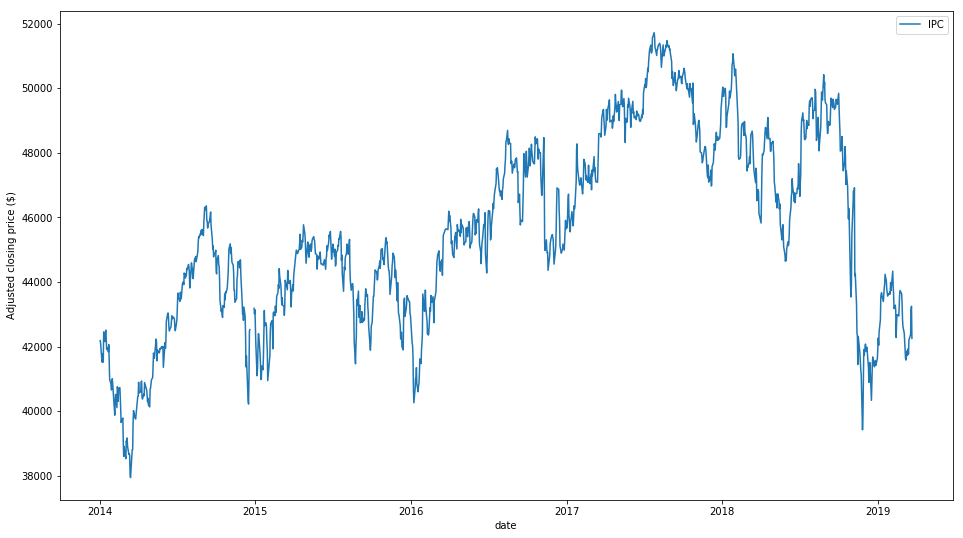
\includegraphics[width=0.45\textwidth]{img/output_6_0.png}
        \caption{Figura 1: Comportamiento del IPC}
        \end{fig2}
        
        
        \subsubsection{Densidad}
        
        Hicimos una función lag con el fin de comporar el cierre de una fecha con la del día anterior, esto de manera porcentual tienen una distribución la cual se observa como sigue.
        
        \begin{fig2}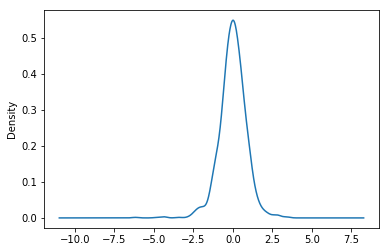
\includegraphics[width=0.45\textwidth]{img/output_8_1.png}
        \caption{Figura 2: La distribución de los cambios día a día.}\end{fig2}
        
        Como se puede observar, dichos incrementos nunca son mayores ni menores a 2.0\%. Por lo que decidimos enfocarnos en estos datos.
        
        \begin{fig2}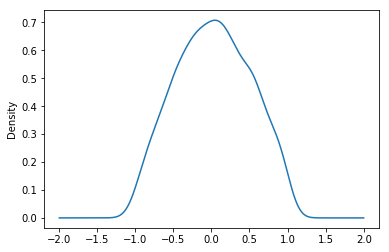
\includegraphics[width=0.45\textwidth]{img/output_9_1.png}
        \caption{Figura 3: Distribución de los cambios el intervalo de cambio [-2.0,  2.0]\end{fig2}
        
        % \subsection{Criterios}
        
        % Para nuestro análisis de sentimiento y su aprendizaje, tendremos 3 sentimientos:
        
        % \begin{itemize}
        %     \item Negativo (-1): cuando el cambio en el IPC de la BMV sea menor o igual a -0.5% respecto al cierre del día anterior
        %     \item Neutral (0): cuando el cambio en el IPC de la BMV sea mayor a -0.5% y menor a +0.5% respecto al cierre del día anterior
        %     \item Positivo (+1): cuando el cambio en el IPC de la BMV sea mayor o igual a +0.5%
        % \end{itemize}

        % Estos números lo tomamos de la distribución de los datos.

        % Nota: se creó una columna, la cual es el posible análisis de sentimiento, el cual posteriormente aplicaremos al modelo de Lenguaje Natural, para intentar extraer el sentimiento basado en el comportamiento del día anterior y los tweets que mencionen palabras clave relacionados con la BMV.

        % Así mismo existen datos faltantes en la información obtenida de Yahoo! Finance.

\subsection{Entrenamiento y prueba}

Para los datos de entrenamietno usamos las primeras 608 observaciones (aproximadamente 75\% de las observaciones) y las observaciones restantes de prueba, no usamos un método aleatorio de selección ya que queremos evitar una filtración de información del conjunto de entrenamiento al de prueba.


\begin{fig2}
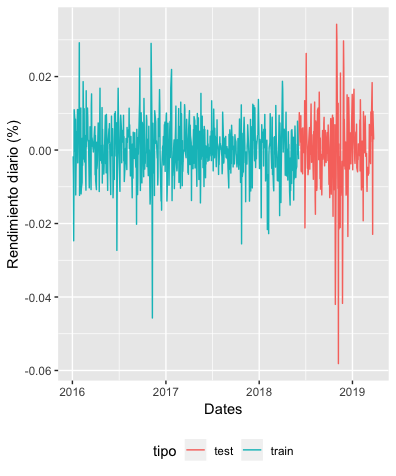
\includegraphics[scale=0.5]{img/IPC_hist.png}
\caption{Figura 4: Retorno histórico del IPC. Conjunto de prueba y entrenamiento}
\end{fig2}

		
\section{Desarrollo}

\subsection{NLP: obtención de los sentimientos}

    Para el análisis de sentimiento se utiliza la librería TextBlob, la cual procesa datos textuales a través del procesamiento de lenguaje natural. Esta librería tiene la gran utilidad de ser basada en NLTK y pattern, con una interfaz más amigable. Algunas de las aplicaciones de la librería son: 
    
    \begin{itemize}
    \item Análisis de sentimiento
    \item Clasificación de Textos
    \item Traducción de textos
    \item Tokenización
    \item N-gramas
    \item Corrección de ortografía ...
    \end{itemize}

    Para el análisis de sentimiento, la librería regresa un par de valores numéricos, el primero relacionado con la Polaridad que está en el rango de [-1.0, 1.0] y la Subjetividad que está en el rango de [0.0 , 1.0] dónde 0.0 es muy objetivo y 1.0 es muy subjetivo. Para propósitos prácticos del análisis se considera que un tweet con Polaridad por abajo de 0 sería negativo y un texto por encima de 0 se consideraría positivo. 
    
\subsubsection{Flujo de extracción}

    Es importante mencionar el flujo de ejecución de los trabajos que se sigue a lo largo de la extracción y análisis de tweets ya que se necesita optimizar ciertos procesos para ahorrar costo computacional, en memoria y tiempo. En primer lugar no se guardan los tweets obtenidos de la plataforma, se prefire por el contrario analizar cada tweet conforme iba entrando al sistema, esto permite que en lugar de tener una colección de textos en memoria, podamos guardar solo una colección de valoraciones numéricas.
    
    Por otro lado, el proceso de Web scrapping del paquete GetOldTweets3 presentaba serios problemas de eficiencia en tiempo, aproximadamente se extraían 10 tweets por minuto, lo cual hacía el proceso bastante largo y sugería que para alcanzar 3 años de 369 tweets diarios tendríamos que correr una máquina en AWS por aproximadamente un mes. 
    
    Este problema se soluciona implementando la manera en que recopilamos los tweets en paralelo por medio de Dask, lo cual permite que se paralelicen lotes de un año, teniendo activos 365 nodos (uno por cada día del año) que a su vez hacen el proceso de Web Scrapping simultáneamente (recopila 369 tweets cada uno). Esto permite que se pueda recolectar la información de un año de actividad en Twitter en 12 horas.
    
    \begin{fig2}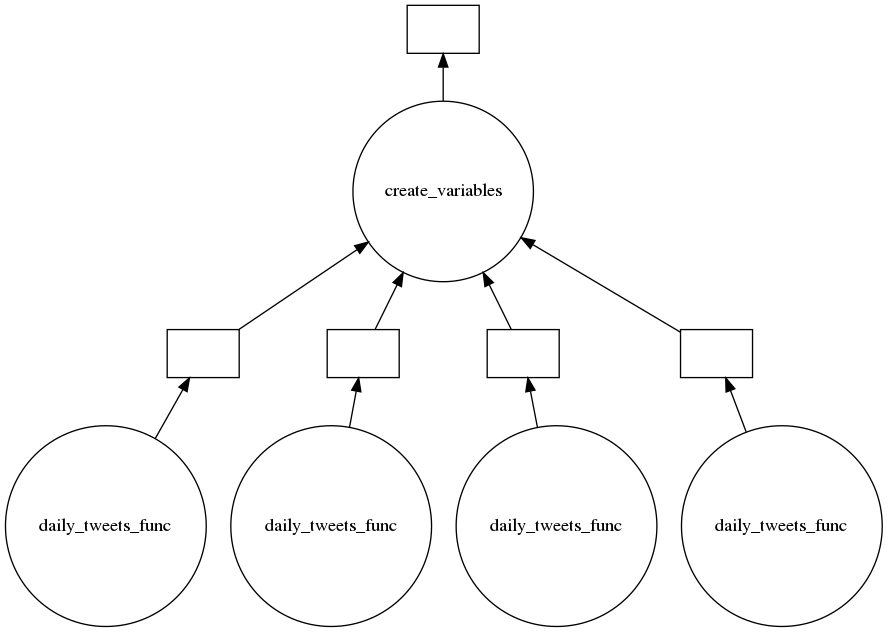
\includegraphics[width=0.35\textwidth]{img/dask_vis.png}
    
    \caption{Figura 5: Diagrama de paralelización en Dask para 4 días.}
    \end{fig2}
    
    
\subsubsection{Preparación de información para análisis}

    Finalmente, el proceso de extracción de tweets en paralelo extrae un archivo csv por día compuesto por un conjunto de tres tweets por cada combinación de los temas y su fuente. Al juntar esta información con otras fechas se observa dos maneras distintas de hacerlo, la primera referente a la forma en la que se presenta la información y la segunda referente a la manera en que los días no laborables fueron tratados. 
    
\subsubsection{Forma de presentar la información}

	Con la información obtenida por el análisis de sentimiento, se construye una matriz donde las  variables independientes $X_{i,j}$ será el ``sentimiento'' aportado por la palabra clave $i$ en el día $j$, y la variable dependiente $R_j$ es el retorno relativo que se obtuvo del IPC en el día $j+1$

    Esta aproximación toma en cuenta las distintas formas en las que la misma información puede ser presentada, esto tiene que ver con el nivel de desglose de los datos. El proyecto utiliza distintos niveles de desgloce siguiendo el siguiente orden; fuente, tema, mezcla de tema y fuente, tema-fuente (nivel mayor de desglose), mezcla de todo (consideramos que incluye información redundante).

\subsubsection{Forma de considerar los días no laborables}

    Aunque se recopila información de todos los días durante tres años, no existe información financiera correspondiente a todos esos días capturados, esto debido a los días no laborables del calendario de la bolsa mexicana de valores. A partir de esta problemática se toma dos distintas aproximaciones: la primera incorpora la información de los días no laborables al día anterior de la predicción, es decir, los tweets del día sábado y domingo se incorporan al análisis de sentimiento del día viernes que será útil para predecir el rendimiento al cierre del día lunes. La segunda aproximación simplemente elimina la información del sentimiento capturado en los días no laborables, es decir, los tweets que se recopilaron en fines de semana se ignoran.

\subsubsection{Unidades de los datos}

    Los datos tienen unidades consistentes a lo largo de cada observación, aunque inicialmente los tweets negativos, positivos y neutros estan representados por el número de apariciones en el día, al incluir la aproximación que incorpora los tweets de los días no laborables se decide expresar el sesgo hacia cierto sentimiento como un porcentaje del total de tweets registrados en ese día. Esta porcentualización del sentimiento hace que los datos queden normalizados en cada observación. 
    
		

\subsection{Cálculo de retorno}
		Utilizamos los datos (de \textit{Yahoo! Finance}) para calcular  el retornos de la siguiente manera $R_t=\frac{P_t-P_{t-1}}{P_{t-1}}$, donde $P_t$ es el precio al tiempo $t$ y $R_t$ es el retorno diario al tiempo $t$. 
\subsection{Modelos}
\subsubsection{Modelo ARIMA(p,d,q)}		
		Utilizamos los datos del inciso 4.2 ajustaremos un modelo ARIMA(p,d,q) para estimar los retornos futuros del IPC. 
		Primero, queremos saber cuantos \textit{lags} Autorregresivos necesitamos, usaremos 2 enfoques. Primero, calcularemos el AIC para los primeros 14 \textit{lags} y obtenemos lo siguiente:

\begin{center}
\begin{tabular}{llllll}
lag & 0     & 1    & 2    & 3    & 4    \\
\hline
AIC & 13.32 & 5.68 & 4.28 & 4.60 & 0.0 
\end{tabular}
\end{center}

\begin{center}
\begin{tabular}{llllll}
lag & 5     & 6    & 7    & 8    & 9    \\
\hline
AIC & 1.78 & 1.04 & 0.68 & 2.66 & 4.17 
\end{tabular}
\end{center}

\begin{center}
\begin{tabular}{llllll}
lag & 10     & 11    & 12    & 13    & 14    \\
\hline
AIC & 5.87 & 7.86 & 9.74 & 11.27 & 13.27 
\end{tabular}
\end{center}

observamos que el AIC es menor para un \textit{lag} de 4. Adicionalmente, si observamos la gráfica de autocorrelaciones observamos que es significativamente distinta de cero hasta el \textit{lag} 4.
\\

\begin{fig2}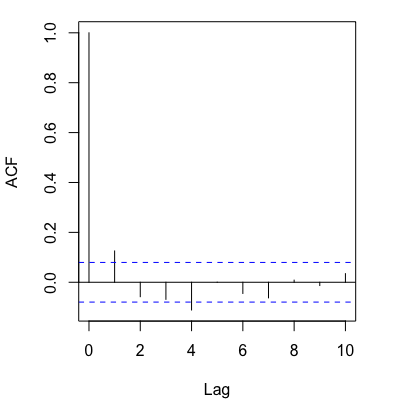
\includegraphics[scale=0.5]{img/ACF.png}
\caption{Figura 6: Gráfica de autocorrelaciones}\end{fig2}
\\
Para identificar el número de \textit{lags} significativos de Medias Móviles utilizamos la Función de Autocorrelaciones Parciales. 

\begin{fig2}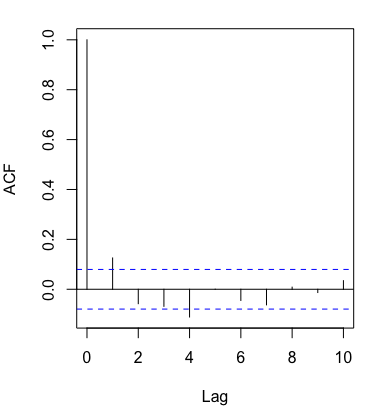
\includegraphics[scale=0.5]{img/PACF.png}
\caption{Figura 7: Gráfica de autocorrelaciones parciales}\end{fig2}

\\\\
Observamos que solamente un \textit{lag} de un periodo anterior es significativamente distinta a cero. \\

Por último, nos interesa saber si es necesario sacar diferencias, para ello obervaremos si los retornos presentan algún tipo de tendencia lineal. 

\begin{fig2}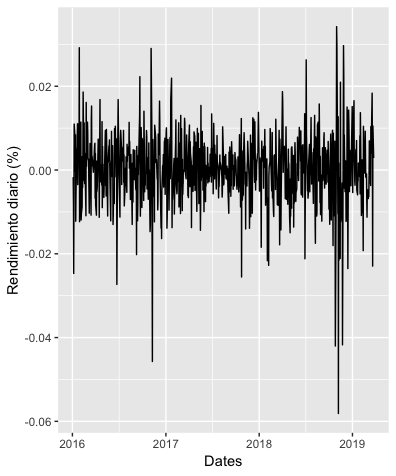
\includegraphics[scale=0.5]{img/IPC.png}
\caption{Figura 8: Gráfica retorno IPC}\end{fig2}
\\\\

En la gráfica anterior notamos que la serie no cuenta con ninguna tendencia lineal y por lo tanto no es necesario sacar diferencias.

Ahora buscamos encontrar los coeficientes correspondinetes a un modelo ARIMA(4,0,1) para los retornos del IPC:

$$R_t-\psi_{t-1}R_{t-1}-\psi_{t-2}R_{t-2}-\psi_{t-3}R_{t-3}-\psi_{t-4}R_{t-4}$$ $$=\mu+\theta_{t-1}\epsilon_{t-1}+\epsilon_t$$

donde $R_t$ es el retorno del IPC en el tiempo $t$, $\epsilon_t$ es el ruido blanco con distribución $N \sim (0, \sigma ^2)$, y $\mu, \psi_{t-1}, \psi_{t-2}, \psi_{t-3}, \psi_{t-4}$ y $\theta_{t-1}$ son los coeficientes que queremos ajustar para el modelo ARIMA.

\begin{center}
\begin{tabular}{llllll}
\multicolumn{6}{l}{Coeficientes ARIMA (4,0,1)}                                          \\
$\psi_{t-4}$           & $\psi_{t-3}$    & $\psi_{t-2}$    & $\psi_{t-1}$    & $\theta{t-1}$         & $\mu$   \\ 
\hline
\uline{-0.12} & \uline{-0.063} & \uline{-0.034} & \uline{-0.188} & \uline{~0.32} & 0.0 
\end{tabular}
\end{center}

Ajustamos los datos del conjunto de prueba al modelo ARIMA y obtuvimos que la suma del error absoluto es 1.905499 y la suma del error cuadrático es 0.03451248.


\subsubsection{Aprendizaje de máquina }

Ahora utilizando los ``sentimientos'' obtenidos a través de los Tweets obtuvimos los siguietes resultados con los distintos modelos.
\begin{itemize}
  \item\textbf{ Regresión Lineal} \\
  Ajustamos un modelo lineal de la siguiente manera $R_t=\beta_0+\beta_1 X_{1,t-1}+...+\beta_p X_{p,t-1}$, donde $R_t$ es el retorno del IPC en el tiempo $t$, y $X_{i,t-1}$ es un sentimiento extraido de los tweets en el tiempo en $t-1$ y $\beta_j$ son los coeficientes estimados para ajustar el modelo. Con este modelo obtenemos una suma del error absoluto de 145,407,833,797.4 y la suma del error cuadrático es $6.16 \times 10^{21}$.
  
  \item \textbf{Regresión Lineal con Regularización Ridge} \\
  Ajustamos un modelo lineal donde buscamos minimizar la siguiente función $D(\beta)=R_t-\beta_0+\beta_1 X_{1,t-1}+...+\beta_p X_{p,t-1}+\lambda \sum_{j=1}^p \beta_j^2$, donde $R_t$ es el retorno del IPC en el tiempo $t$, y $X_{i,t-1}$ es un sentimiento extraido de los tweets en el tiempo en $t-1$, $\beta_j$  son los coeficientes estimados para ajustar el modelo y $\lambda$ es el factor de regularización Ridge. Con este modelo obtenemos una suma del error absoluto de 1.6338 y la suma del error cuadrático es 0.02612. Adicionalmente, podemos observar que los residuales del modelo parecen tener una distribución $N \sim (0,\sigma ^2).$
  \\\\
 \begin{fig2}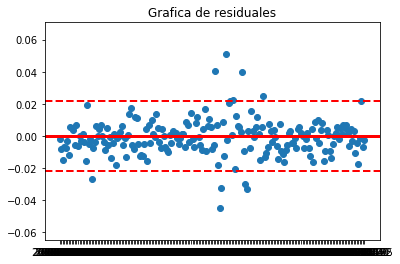
\includegraphics[scale=0.5]{img/Residuales_ridge.png}
 \caption{Figura 9: Gráfica de residuales del modelo de regresión lineal con regularización Ridge}\end{fig2}

  \item \textbf{Regresión Lineal con Regularización Lasso} \\
  Ajustamos un modelo lineal donde buscamos minimizar la siguiente función $D(\beta)=R_t-\beta_0+\beta_1 X_{1,t-1}+...+\beta_p X_{p,t-1}+\lambda \sum_{j=1}^p |\beta_j |$, donde $R_t$ es el retorno del IPC en el tiempo $t$, y $X_{i,t-1}$ es un sentimiento extraído de los tweets en el tiempo en $t-1$, $\beta_j$  son los coeficientes estimados para ajustar el modelo y $\lambda$ es el factor de regularización Lasso. Con este modelo obtenemos una suma del error absoluto de 1.5964 y la suma del error cuadrático es 0.02488. Adicionalmente, podemos observar que los residuales del modelo parecen tener una distribución $N \sim (0,\sigma ^2).$
    \\
 \begin{fig2}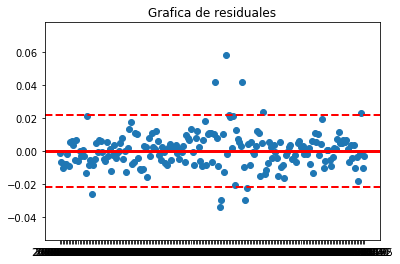
\includegraphics[scale=0.5]{img/Residuales_lasso.png}
 \caption{Figura 10: Gráfica de residuales del modelo de regresión lineal con regularización Lasso}\end{fig2}

  \item \textbf{Bosques aleatorios} \\
  Con un modelo de 100 árboles aleatorios obtenemos una suma del error absoluto de 1.6928 y la suma del error cuadrático es 0.02662. Podemos observar las proyecciones de los retornos vs. el valor real en la gráfica inferior.
      \\
 \begin{fig2}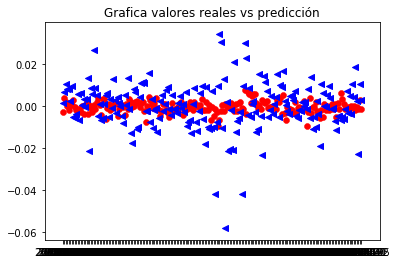
\includegraphics[scale=0.5]{img/Proy_RF.png}
 \caption{Figura 11: Retornos real del IPC vs. predicción del modelo de bosques aleatorios}\end{fig2}
  
  \item \textbf{XGboost} \\
 Ajustamos un modelo XGboost el cual nos dió el mejor rendimiento con los siguientes parámetros 60 árboles, máxima profundidad de 1 y con un parámetro de regularización de 0.1, y obtuvimos una suma del error absoluto de 1.5954 y la suma del error cuadrático es 0.02492. 
 
 \item \textbf{K-vecinos más cercanos} \\
Con un modelo de 10 vecinos más cercanos obtuvimos una suma del error absoluto de 1.6333 y la suma del error cuadrático es 0.02614. 

\end{itemize}


		\section{Conclusión}	
	Como podemos observar en la tabla de Resultados en todos los modelos de Aprendizaje de Máquina, menos el de Regresión Lineal, los modelos tienen un \textit{performance} mejor (en terminos de la suma de diferencia de cuadrados y de suma de diferencias de valor absoluto) que el modelo ARIMA, es decir, la información extraida de los tweets usando técnicas de Aprendizaje de Máquina nos dió mejores resultados que usar la información histórica de los datos con un modelo ARIMA.
	
	Sin atribuir causalidad, podemos decir que los resultados se muestran mucho más sólidos con análisis de sentimiento dado que se puede decir que aportan información que enriquece modelos de aprendizaje máquina. Esto es detallado en la bibliografía de este proyecto, pues menciona Jurafsky que aunque el análisis de sentimiento no es exacto, sí puede aportar cierta dirección. 
	
	Por una parte XGBoost pudiera tener una fortaleza con datos dispersos, de acuerdo a lo descrito en el paper original que publicó el método \cite{xgb}. Por otra parte lasso podría considerarse con características similares, tales como \textit{encogimiento} y \textit{selección de variables}, como lo menciona el Dr. Luis Felipe González\cite{luisfelipe}. 
	

\begin{center}
\caption{Tabla: Resultados}
\centering
\begin{tabular}{ll|l}
                       & \multicolumn{2}{l}{Suma de las diferencias}         \\ 
\cline{2-3}
Método                 & \multicolumn{1}{l|}{Valor Absoluto} & Cuadrado      \\ 
\cline{2-3}
ARIMA (4,0,1)          & 1.905499                            & 0.0345124     \\
Regresión Lineal       & $1.45\times10^{11}$                 & $6.16 \times 10^{21}$  \\
Regresión Ridge        & 1.6338                              & 0.02612       \\
Regresión Lasso        & 1.5964                              & \cellcolor[HTML]{C9CFEC} 0.02488       \\
Bosques aleatorios     & 1.6928                              & 0.02662       \\
XGBoost                & \cellcolor[HTML]{C9CFEC}1.5954                              & 0.02492       \\
K-vecinos \\ más cercanos & 1.6333                              & 0.02614                   
\end{tabular}
\end{center}
	\end{multicols}
	
	
	\begin{thebibliography}{1}

	\bibitem{meucci} 
	Meucci, Attilio.
	\textit{'P' Versus 'Q': Differences and Commonalities between the Two Areas of Quantitative Finance (January 22, 2011)}. GARP Risk Professional, pp. 47-50, February 2011.

	\bibitem{danj}Dan Jurafsky, James H. Martin. \textit{Speech and Language Processing (3rd ed. draft)}. Prentice-Hall. Septiembre 23, 2018.
	
	\bibitem{velay}Marc Velay, Fabrice Daniel. Using NLP on news headlines to predict index trends. Artificial Intelligence Department of Lusis, Paris, France. arXiv:1806.09533
	
	\bibitem{guerrero}Victor Guerrero. Análisis estadístico y pronóstico de series de tiempo económicas. Ciudad de México. México. Justin time press. 2009.
	
	\bibitem{xgb}Tianqi Chen, Carlos Guestrin. XGBoost: A Scalable Tree Boosting System. Version 3. University of Washington. 2016. arXiv:1603.02754
	
	\bibitem{luisfelipe}Luis Felipe González-Pérez. Curso de Aprendizaje de máquina. Instituto Tecnológico Autónomo de México. 2019. https://felipegonzalez.github.io/aprendizaje-maquina-2017/
	\end{thebibliography}
\end{document}